\clearpage{}

\section{Cite and briefly describe, with small examples, the types of
notation that can be used to describe the structure, the behaviour or the
functions of a system. Define and distinguish the notions of verification
and validation, and the techniques that can apply to them. Explain how
they apply to requirements.}

\subsection{Types of notation to describe the structure, the behaviour or the functions
of a system}

\begin{itemize}
    \item \textbf{Structure}
        \begin{itemize}
            \item Entity-Relationship diagram (ER diagram)
            \item Class diagram
        \end{itemize}

    \item \textbf{Behaviour}
        \begin{itemize}
            \item Event traces
            \item Sequence diagram
            \item State Machine
            \item Statechart Diagram
            \item Petri nets
            \item Data-flow diagram
            \item Use-case diagram
        \end{itemize}

    \item \textbf{Functions}
        \begin{itemize}
            \item Decision table
            \item Parnas table
            \item Object constraint language (OCL)
            \item Algebraic specifications
        \end{itemize}
\end{itemize}


\subsection{Notions of verification and validation}

\begin{description}
    \item[Verification] Specifications conform to requirements (i.e. \enquote{build the right system})
        \subitem{} $\rightarrow$ documents $\div$ documents
        (\textcolor{green!80!black}{easier})
    \item[Validation] Requirements accurately reflects the customer's needs (i.e. \enquote{build the system right})
        \subitem{} $\rightarrow$ needs $\div$ documents (\textcolor{red!80!black}{harder})
\end{description}

\begin{figure}[!ht]
    \centering
    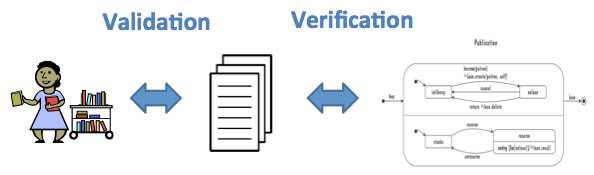
\includegraphics[width=0.6\linewidth]{validation_verification.png}
    \caption{Validation and verification}
\end{figure}
\FloatBarrier{}

\subsubsection{How they apply to requirements}

\begin{table}[!ht]
    \begin{center}
        \begin{tabular}{cc}
            \toprule
            Verification            & Validation \\
            \midrule
            Cross-referencing       & Walkthrough \\
            Simulation              & Readings \\
            Consistency checks      & Interviews \\
            Completeness checks     & Reviews \\
            Reachability checks (states, transitions) & Checklists \\
            Model checking          & Formal inspections \\
            Mathematical proofs     & Modeling \\
                                    & Scenarios \\
                                    & Prototypes \\
                                    & Simulation \\
            \bottomrule
        \end{tabular}
    \end{center}
    \caption{Technique that apply to verification and validation}
\end{table}

\begin{itemize}

\item \textbf{Verification}

Check that specifications are conforming to definitions and to other specifications (consistency). 
\begin{itemize} 
    \item Check traceability (between requirement/spec/design/implem/verif) or better demonstrate.
        \begin{center}
            Specification \textbf{AND} assumptions \textbf{IMPLY} requirements
        \end{center}
    \item Eventually computer helped (model checking or theorem proving).
\end{itemize}

\item \textbf{Validation}

    Review of the requirements by representatives of the customer and the developer. Meeting to discuss the result. 

    \begin{tabular}{cm{10cm}}
        Steps:&
        \begin{enumerate}
            \item Review the goals and objectives of the system
            \item Compare requirement with goal and objectives
            \item Review environment in which the system operates
            \item Review the information flow and proposed function
            \item Asses and document risk, discuss and compare
                alternative 
            \item Discuss how requirements will be tested
        \end{enumerate}
    \end{tabular}
\end{itemize}
